\section*{Dynamic Test Specification}

In the Waterfall model we have chosen includes a testing in phase 4. After developers have developers are done with coding and provide final build to testers, testing starts in this phase. Through this phase we intend to reflect on the following points:

\subsection*{Test planning}
In the test planning we will decide what we want to test, define the test process, schedule the testing, estimate testing effort and assign testing resources. We will further consider how to report the test result and how they are handled

\subsection*{Design of test cases}
In our test cases we intend to include a unique identification, execution preconditions, data and actions inputs, our expected results and finally trace the individual tasks. These task will be done in a systematic manner.

\subsection*{Prepare Test Data}
At this stage of the process we will prepare the data which we intend to test

\subsection*{Prepare Test Environment}
At this stage of the process we intend to prepare the test environment. In the testing environment for our case, we are going to prepare a computer as the server. It supports to running all the time during the test. We also need a card reader machine and a mobile phone. They all have the internet accessed. 
On the server, it is running the server program and test program. The card reader machine and mobile should run the client program.

\subsection*{Run Program on Test Data}
The test program can monitor the client side(card reader machines and mobile app) if connect to the server and the data return back to the server. And it also can monitor the input and output data on the server.

\subsection*{Compare Results to Test Cases}
In our case, when we run the test program on the server, we will get the output as data. We see if the data as what we expected.

\subsection*{Report Testing}
We put all the testing data as log that saves in the server.

\subsection*{Correct Errors}
If the output data is not what we expected, we will find the errors and fix it.

Our overall process can be summarized in the figure seen below, which is a traditional testing process.

\begin{figure}[ht!]
	\centering
	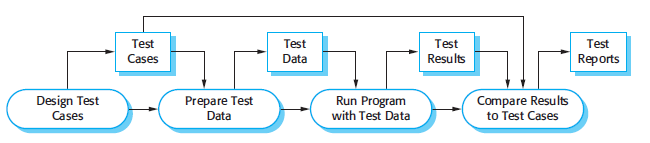
\includegraphics[width=90mm]{graphics/dynamic_test_specification.png}
	\label{overflow}
\end{figure}


\subsection*{Test Cases}

\subsubsection*{Test Case 1: Check In - Card}
\begin{enumerate}
	\item ID
		\begin{enumerate}
			\item TC1
		\end{enumerate}
	\item Pre-con
		\begin{enumerate}
			\item System ready for card input
			\item Connected to the server
			\item The card should be functional
			\item There is money on the card/account
		\end{enumerate}
	\item Input
		\begin{enumerate}
			\item Data from the card
		\end{enumerate}
	\item Expected result
		\begin{enumerate}
			\item Ok message indicating that the check-in was successful 
		\end{enumerate}
\end{enumerate}


\subsubsection*{Test Case 2: Check In - Mobile}
\begin{enumerate}
	\item ID
		\begin{enumerate}
			\item TC2
		\end{enumerate}
	\item Pre-con
		\begin{enumerate}
			\item System ready for card input
			\item Connected to the server
			\item The mobile app should be functional
			\item There is money in the account
		\end{enumerate}
	\item Input
		\begin{enumerate}
			\item Data from the mobile app
		\end{enumerate}
	\item Expected result
		\begin{enumerate}
			\item Ok message indicating that the check-in was successful 
		\end{enumerate}
\end{enumerate}


\subsubsection*{Test Case 3: Check Out(card)}
\begin{enumerate}
	\item ID
		\begin{enumerate}
			\item TC3
		\end{enumerate}
	\item Pre-con
		\begin{enumerate}
			\item System ready for card input
			\item Connected to the server
			\item The card should be functional
		\end{enumerate}
	\item Input
		\begin{enumerate}
			\item Data from the card
		\end{enumerate}
	\item Expected result
		\begin{enumerate}
			\item Ok message indicating that the check-in was successful 
		\end{enumerate}
\end{enumerate}


\subsubsection*{Test Case 4: Add Balance}
\begin{enumerate}
	\item ID
		\begin{enumerate}
			\item TC4
		\end{enumerate}
	\item Pre-con
		\begin{enumerate}
			\item Connected to the server
			\item The account should be valid and functioning
			\item Internet must be accessible
		\end{enumerate}
	\item Input
		\begin{enumerate}
			\item Account transformation from the user's bank account to the travel card system
		\end{enumerate}
	\item Expected result
		\begin{enumerate}
			\item Updated user credit in the travel card system
		\end{enumerate}
\end{enumerate}



\subsubsection*{Test Case 5: Check Customer Status}
\begin{enumerate}
	\item ID
		\begin{enumerate}
			\item TC5
		\end{enumerate}
	\item Pre-con
		\begin{enumerate}
			\item Connected to the server
			\item The system should be functional
		\end{enumerate}
	\item Input
		\begin{enumerate}
			\item Users travel card or app
		\end{enumerate}
	\item Expected result
		\begin{enumerate}
			\item Status of whether the user is checked in or not
		\end{enumerate}
\end{enumerate}
